Das Ursprüngliche Ziel des Projektes war es, eine Drohne mittels Bewegungssteuerung zu Steuern.\\
Im Laufe des Projektes haben wir jedoch schnell festgestellt, dass dies in der kurzen Zeit und mit unserer begrenzten Erfahrung nicht möglich ist.
Um unser System trotzdem testen zu können, haben wir uns dazu entschieden ein kleines Demo-Game zu entwickeln.\\
Das Game wurde mit Unity3D erstellt, die Kommunikation mit dem Controller funktioniert über eine Serielle Schnittstelle und unserem eigenen Kleinen Protokoll.
Dabei war es uns wichtig, dass das die Kommunikation bidirektional erfolgen kann. Das heisst das der Benutzer mit dem Controller das Spiel steuern aber im Game den
Controller auch konfigurieren kann.\\

\subsubsection{Hauptmenü}
Nach dem Start des Games wird das Game Hauptmenü angezeigt. Hier muss über ''Connect'' zuerst die Verbindung mit dem Arduino hergestellt werden. Anschliessend kann man das Game starten oder über ''PID-Setup'' die PID's auf dem Arduino anpassen.

\begin{figure}[H]
  \begin{center}
    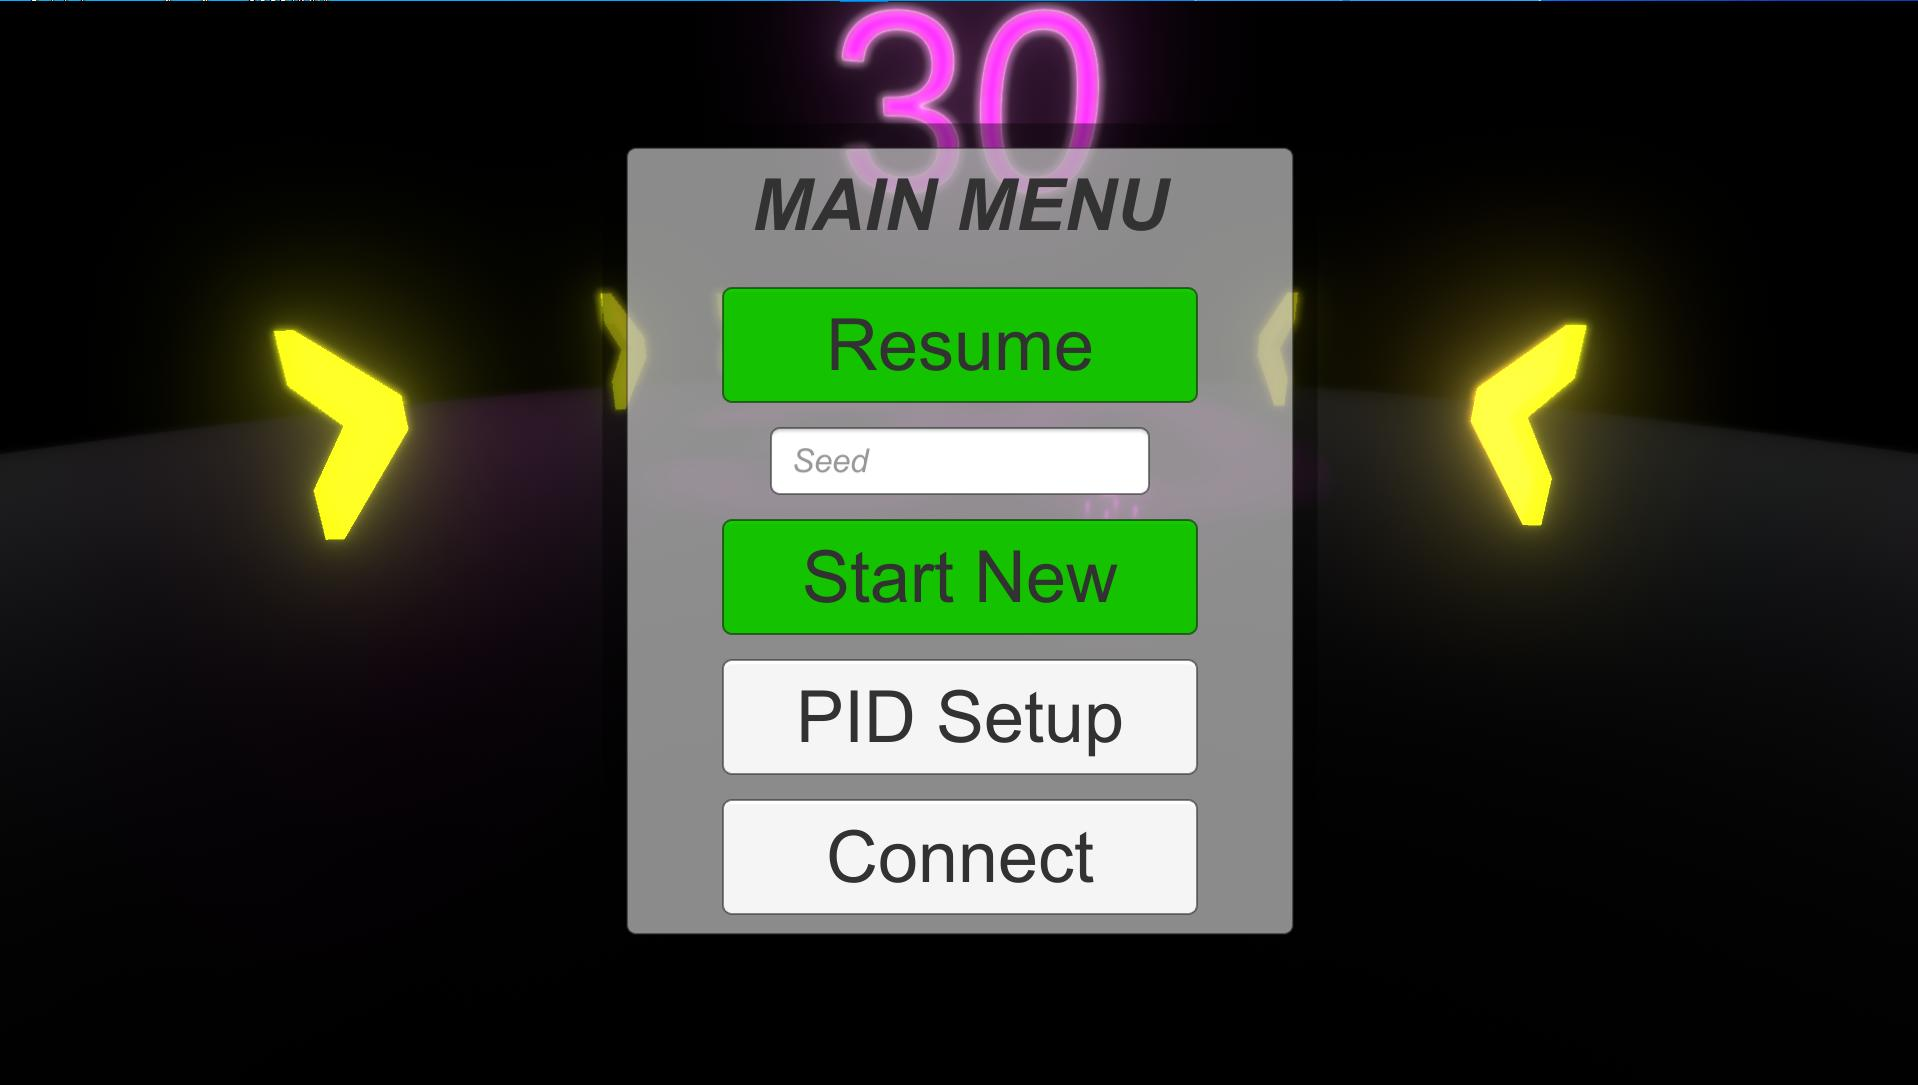
\includegraphics[width=0.55\linewidth]{content/images/menu1.jpg}
    \caption{Game Hauptmenü}
  \end{center}
\end{figure}

\newpage
\subsubsection{Verbindung herstellen}
In diesem Submenü wird die Verbindung zum Arduino hergestellt. Dazu muss der richtige COM-Port eingegeben werden, ansonsten kann die Verbindung nicht aufgebaut werden. Ist das herstellen der Verbindung erfolgreich, wird in der Statusleiste oben angezeigt, dass das Gyro Kalibriert wird. Währenddessen darf der Arduino nicht bewegt werden.
\begin{figure}[H]
  \begin{center}
    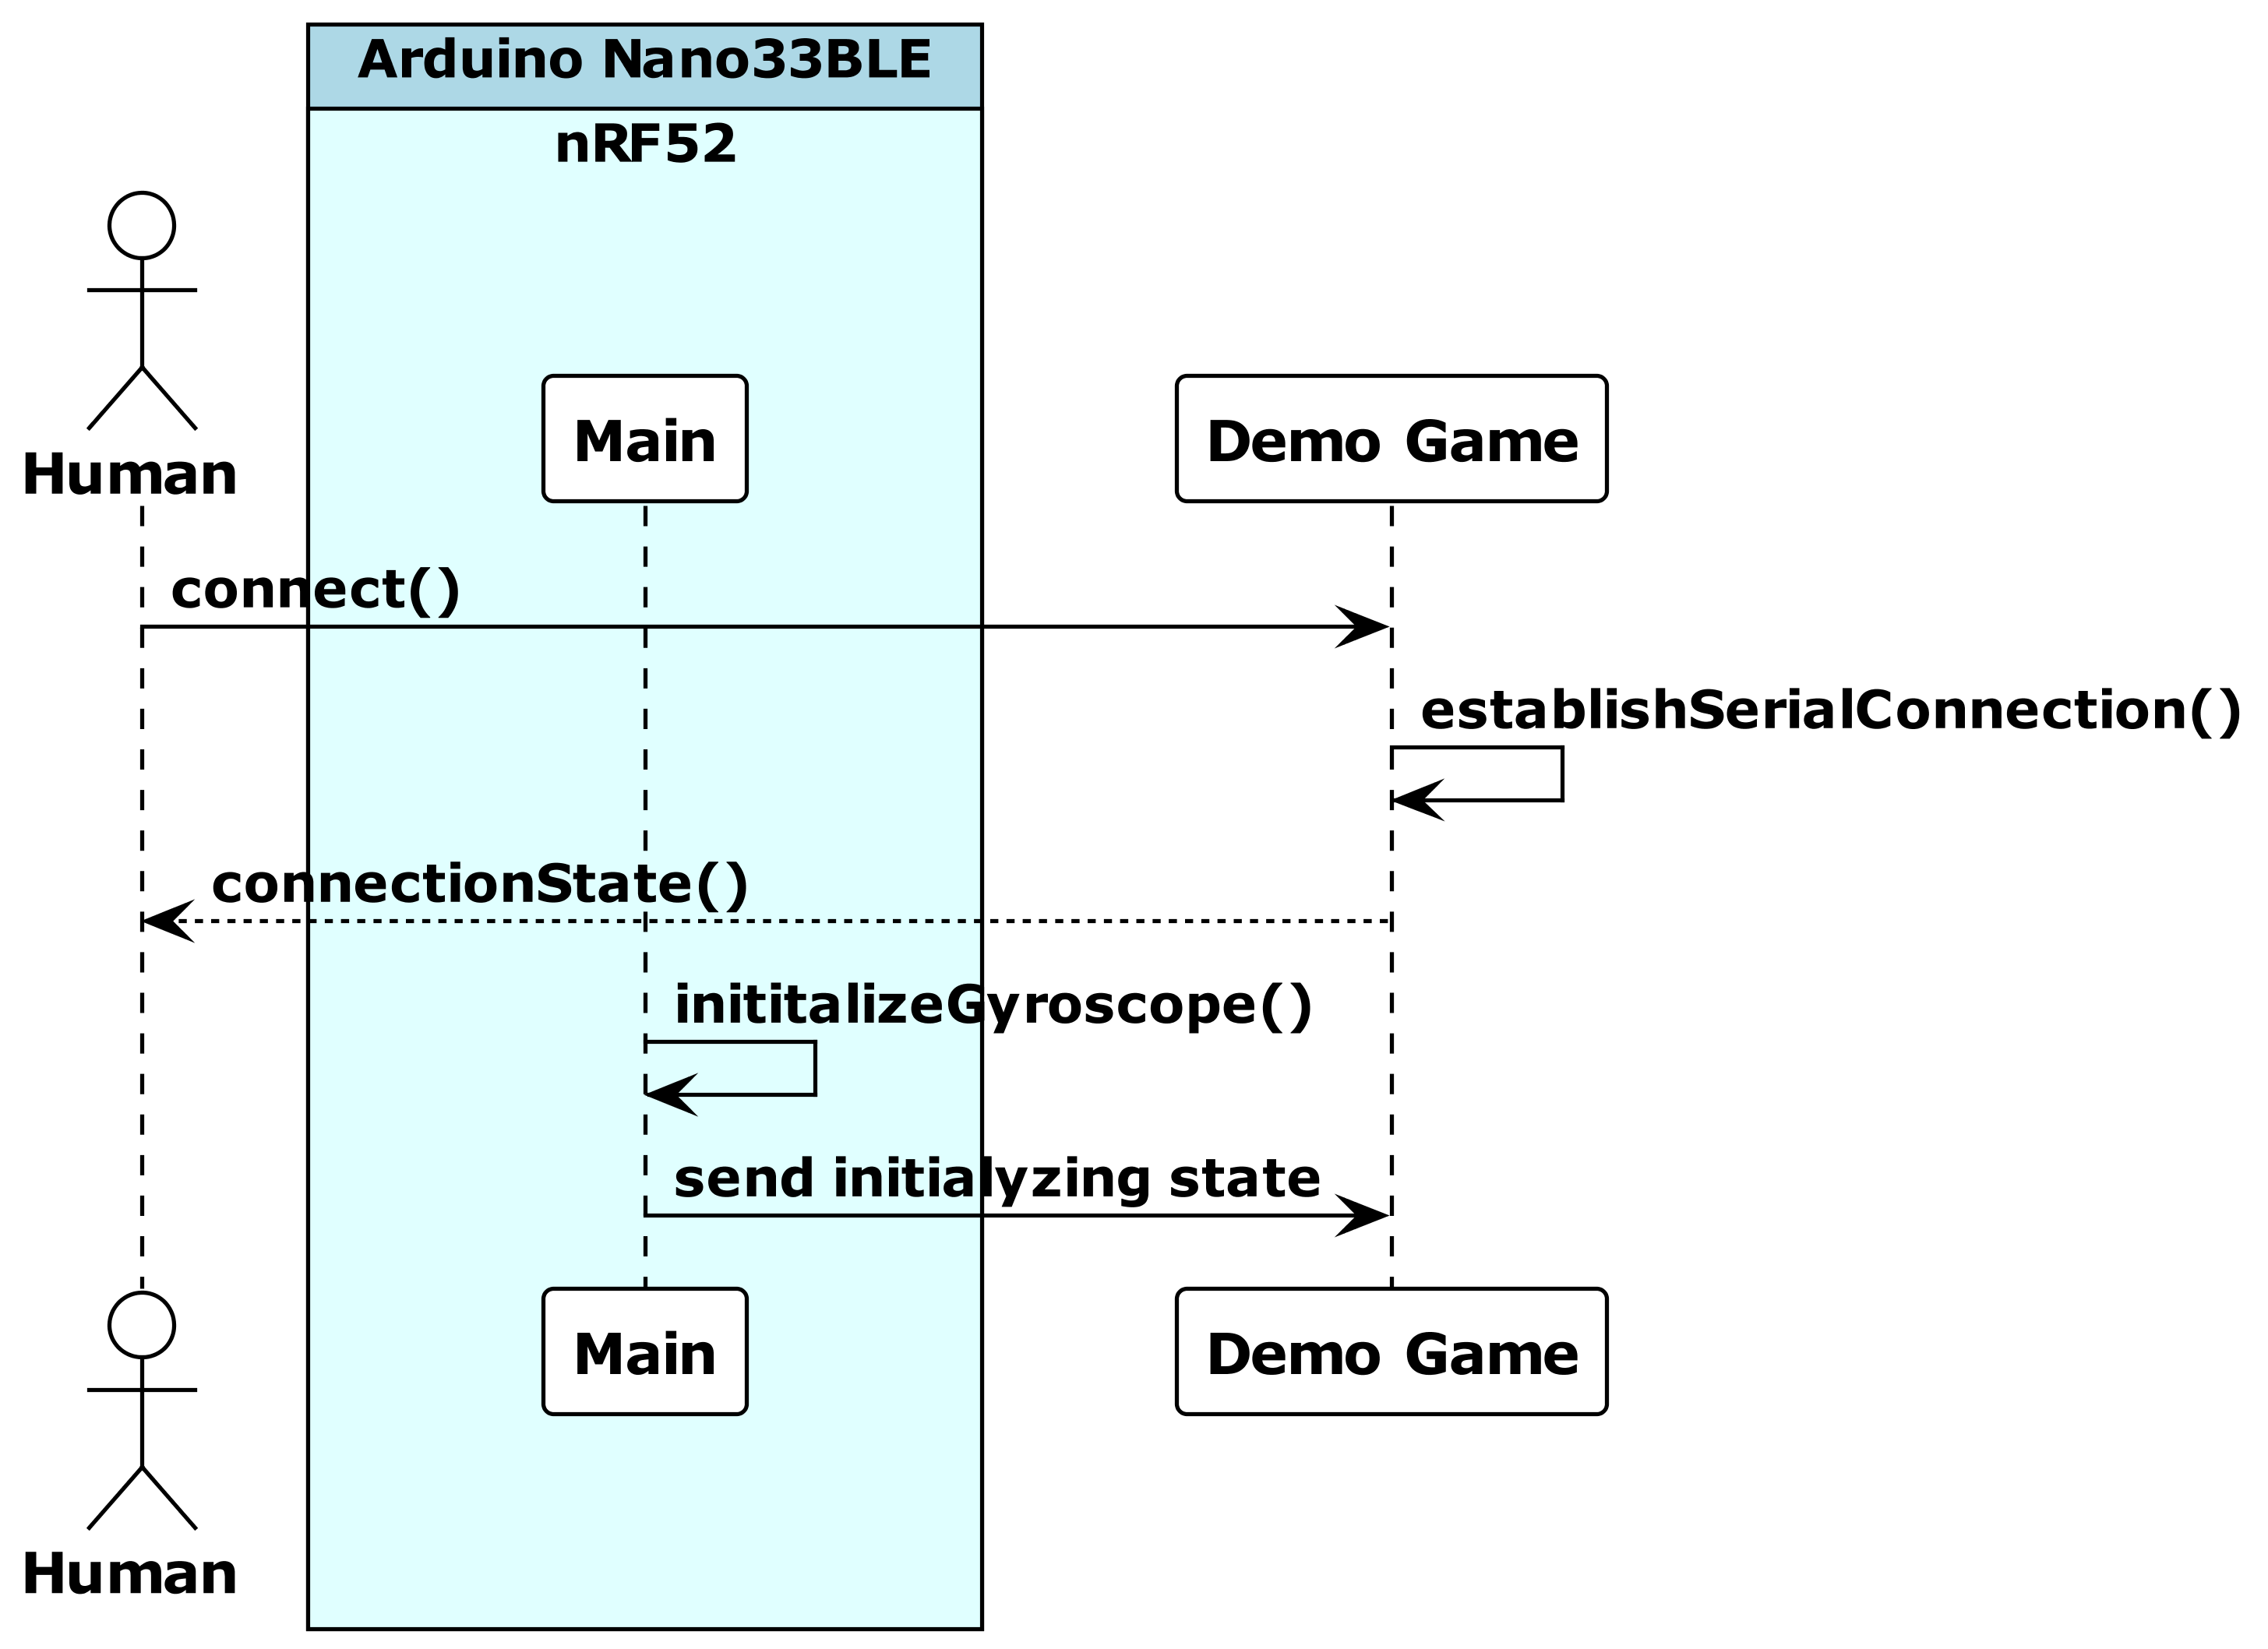
\includegraphics[width=0.45\linewidth]{content/images/connect.jpg}
    \caption{Verbindung herstellen}
  \end{center}
\end{figure}

\subsubsection{PID-Setup}
Falls man die voreingestellten Werte der PID-Konstanten anpassen möchte, kann man dies hier über das PID-Setup machen. Zuerst müssen die aktuellen Werte vom Arduino mit ''Reload'' geladen werden, danach können diese mit ''Apply'' auf den Arduino geschrieben werden.
\begin{figure}[H]
  \begin{center}
    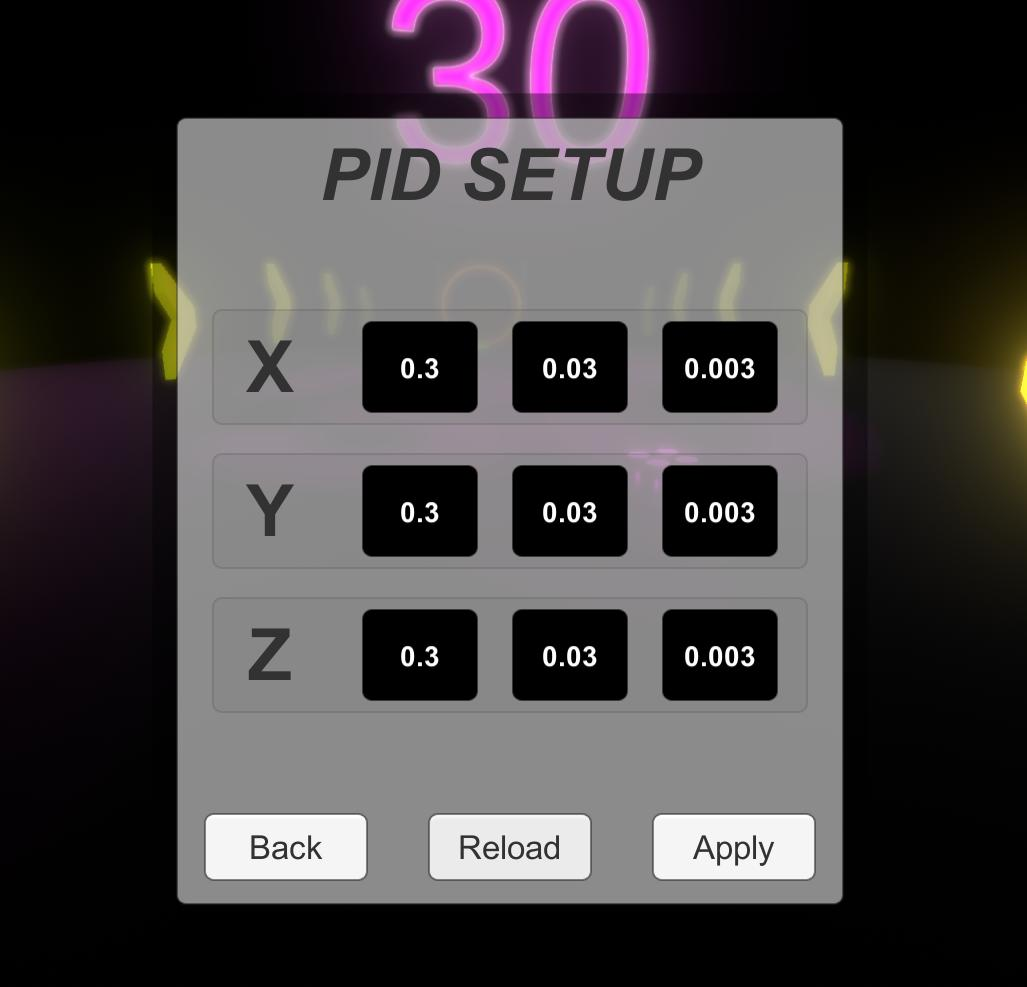
\includegraphics[width=0.45\linewidth]{content/images/PID.jpg}
    \caption{PID Einstellen}
  \end{center}
\end{figure}

\newpage
\subsubsection{Gameziel}
Wenn die Verbindung erfolgreich hergestellt wurde, kann ein neues Game gestartet werden. Durch kippen des Arduino nach vorne fliegt die Drohne vorwärts und dann muss versucht werden durch die eingeblendeten Tore hindurchzufliegen.
\begin{figure}[H]
  \begin{center}
    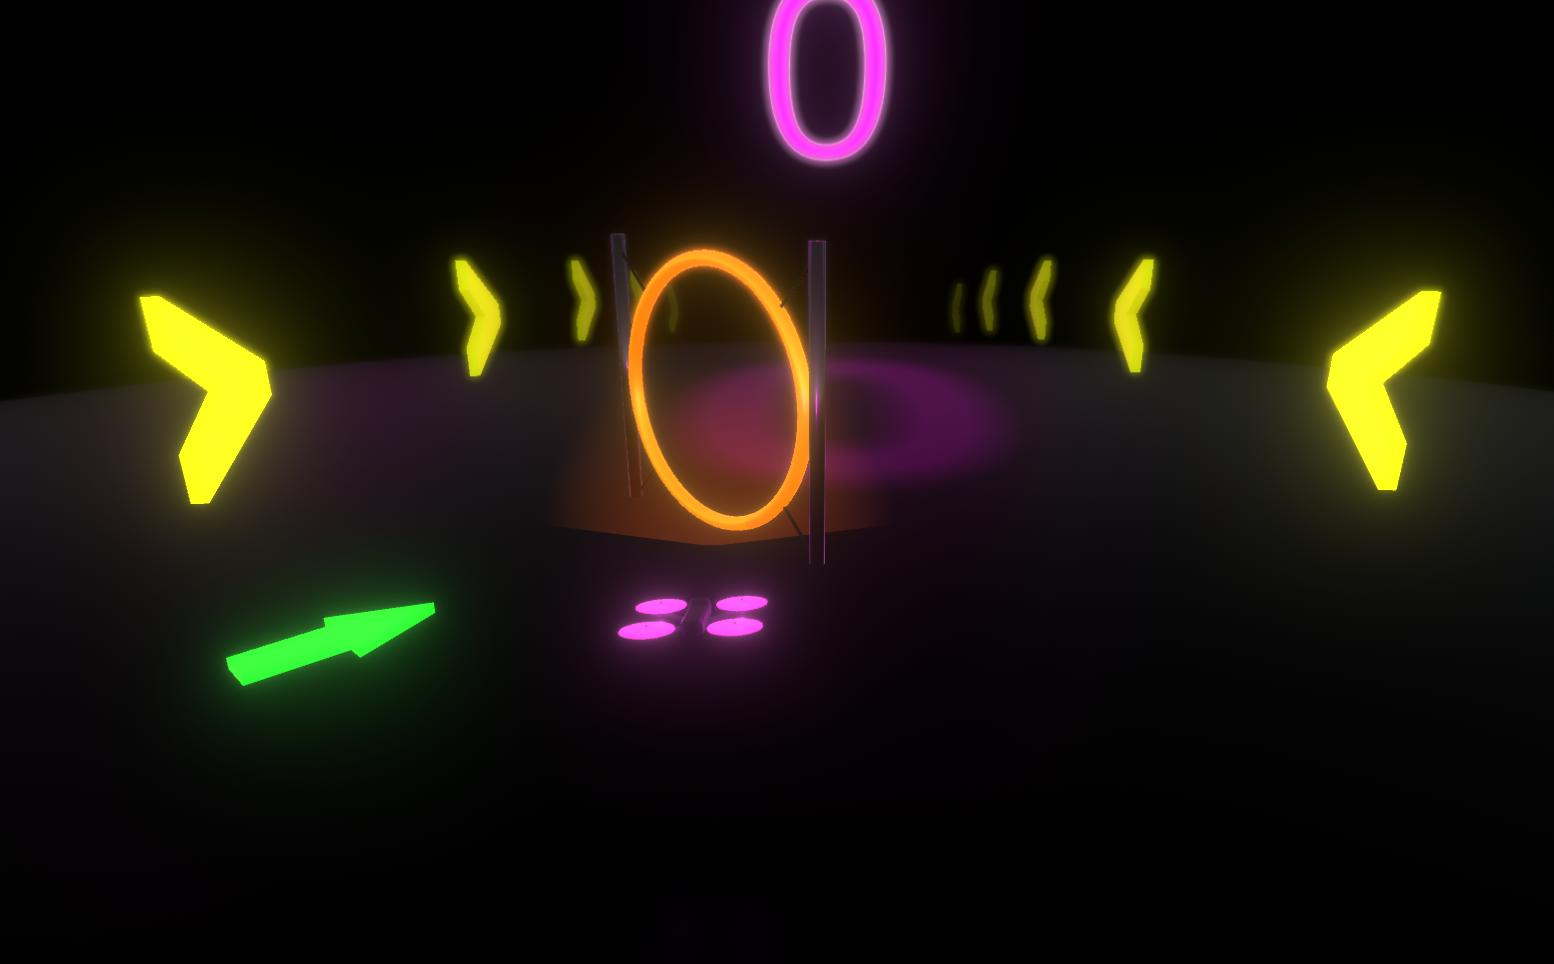
\includegraphics[width=0.6\linewidth]{content/images/game.jpg}
    \caption{In-Game Screenshot}
  \end{center}
\end{figure}